%%%%%%%%%%%%%%%%%%%%%%%%%%%%%%%%%%%%%%%%%
% Short Sectioned Assignment LaTeX Template Version 1.0 (5/5/12)
% This template has been downloaded from: http://www.LaTeXTemplates.com
% Original author:  Frits Wenneker (http://www.howtotex.com)
% License: CC BY-NC-SA 3.0 (http://creativecommons.org/licenses/by-nc-sa/3.0/)
%%%%%%%%%%%%%%%%%%%%%%%%%%%%%%%%%%%%%%%%%

% \documentclass[paper=a4, fontsize=11pt]{scrartcl} % A4 paper and 11pt font size
\documentclass[12pt, a4paper, openany]{book}
\usepackage[T1]{fontenc} % Use 8-bit encoding that has 256 glyphs
\usepackage{fourier} % Use the Adobe Utopia font for the document - comment this line to return to the LaTeX default
\usepackage[utf8]{inputenc}
\usepackage{listings} % para insertar código con formato similar al editor
\usepackage[spanish, es-tabla]{babel} % Selecciona el español para palabras introducidas automáticamente, p.ej. "septiembre" en la fecha y especifica que se use la palabra Tabla en vez de Cuadro
\usepackage{url} % ,href} %para incluir URLs e hipervínculos dentro del texto (aunque hay que instalar href)
\usepackage{graphics,graphicx, float} %para incluir imágenes y colocarlas
\usepackage[gen]{eurosym} %para incluir el símbolo del euro
\usepackage{cite} %para incluir citas del archivo <nombre>.bib
\usepackage{enumerate}
\usepackage{hyperref}
\usepackage{graphicx}
\usepackage{tabularx}
\usepackage{booktabs}

\usepackage[table,xcdraw]{xcolor}
\hypersetup{
	colorlinks=true,	% false: boxed links; true: colored links
	linkcolor=black,	% color of internal links
	urlcolor=cyan		% color of external links
}
\usepackage{fancyhdr} % Custom headers and footers
\pagestyle{fancyplain} % Makes all pages in the document conform to the custom headers and footers
\fancyhead[L]{} % Empty left header
\fancyhead[C]{} % Empty center header
\fancyhead[R]{Sheila Martínez Gómez} % My name
\fancyfoot[L]{} % Empty left footer
\fancyfoot[C]{} % Empty center footer
\fancyfoot[R]{\thepage} % Page numbering for right footer
%\renewcommand{\headrulewidth}{0pt} % Remove header underlines
\renewcommand{\footrulewidth}{0pt} % Remove footer underlines
\setlength{\headheight}{13.6pt} % Customize the height of the header
%\renewcommand{\familydefault}{\sfdefault}
\usepackage{titlesec, blindtext, color}


\definecolor{gray75}{gray}{0.75}
\definecolor{lightpurple}{HTML}{eeddff}
\definecolor{deeppurple}{HTML}{c58cff}

\newcommand{\hsp}{\hspace{20pt}}
\titleformat{\chapter}[hang]{\Huge\bfseries}{\thechapter\hsp\textcolor{gray75}{|}\hsp}{0pt}{\Huge\bfseries}
\setcounter{secnumdepth}{4}
\usepackage[Bjornstrup]{fncychap}

\renewcommand\DOCH{%
  \settowidth{\py}{\CNoV\thechapter}
  \addtolength{\py}{-10pt}
  \fboxsep=0pt%
  \colorbox{lightpurple}{\rule{0pt}{40pt}\parbox[b]{\textwidth}{\hfill}}%
  \kern-\py\raise20pt%
  \hbox{\color{deeppurple}\CNoV\thechapter}\\%
}

\renewcommand\DOTI[1]{%
  \nointerlineskip\raggedright%
  \fboxsep=\myhi%
  \vskip-1ex%
  \colorbox{lightpurple}{\parbox[t]{\mylen}{\CTV\FmTi{#1}}}\par\nobreak%
  \vskip 40pt%
}

\renewcommand\DOTIS[1]{%
  \fboxsep=0pt
  \colorbox{lightpurple}{\rule{0pt}{40pt}\parbox[b]{\textwidth}{\hfill}}\\%
  \nointerlineskip\raggedright%
  \fboxsep=\myhi%
  \colorbox{lightpurple}{\parbox[t]{\mylen}{\CTV\FmTi{#1}}}\par\nobreak%
  \vskip 40pt%
 }


\begin{document}

	% Plantilla portada UGR
	\begin{titlepage}
\newlength{\centeroffset}
\setlength{\centeroffset}{-0.5\oddsidemargin}
\addtolength{\centeroffset}{0.5\evensidemargin}
\thispagestyle{empty}

\noindent\hspace*{\centeroffset}\begin{minipage}{\textwidth}

\centering

\includegraphics[width=0.9\textwidth]{logos/logo_ugr.jpg}\\[1.4cm]

\textsc{ \Large TRABAJO FIN DE GRADO\\[0.2cm]}
\textsc{ GRADO EN INGENIERIA INFORMATICA}\\[1cm]

\center{\Huge\bfseries Control de elementos  }
\center{\Huge\bfseries de un automóvil mediante}
\center{\Huge\bfseries  un sistema empotrado} 
\noindent\rule[-1ex]{\textwidth}{1pt}\\[3.5ex]

\end{minipage}

\vspace{2.5cm}
\noindent\hspace*{\centeroffset}
\begin{minipage}{\textwidth}
\centering

\textbf{Autor}\\ {Sheila Martínez Gómez}\\[2.5ex]
\textbf{Director}\\ {Jesús González Peñalver}\\[2cm]

\includegraphics[width=0.3\textwidth]{logos/etsiit_logo.png}\\[0.1cm]
\textsc{Escuela Técnica Superior de Ingenierías Informática y de Telecomunicación}\\

\end{minipage}
\end{titlepage}


	% Plantilla prefacio UGR
	\thispagestyle{empty}

\begin{center}
{\large\bfseries Control de elementos de un automóvil \\ mediante un Sistema Empotrado }\\
\end{center}
\begin{center}
Sheila Martínez Gómez\\
\end{center}

%\vspace{0.7cm}

\vspace{0.5cm}
\noindent\textbf{Palabras clave}: \textit{software libre, sistema empotrado, ECU, microcontrolador, centralita, RTOS, automoción}
\vspace{0.7cm}

\noindent\textbf{Resumen}\\
	

\cleardoublepage

\begin{center}
	{\large\bfseries Same, but in English}\\
\end{center}
\begin{center}
	Student's name\\
\end{center}
\vspace{0.5cm}
\noindent\textbf{Keywords}: \textit{open source, embedded system, ECU, microcontroller,RTOS, automotive}, \textit{floss}
\vspace{0.7cm}

\noindent\textbf{Abstract}\\


\cleardoublepage

\thispagestyle{empty}

\noindent\rule[-1ex]{\textwidth}{2pt}\\[4.5ex]

D. \textbf{Tutora/e(s)}, Profesor(a) del ...

\vspace{0.5cm}

\textbf{Informo:}

\vspace{0.5cm}

Que el presente trabajo, titulado \textit{\textbf{Chief}},
ha sido realizado bajo mi supervisión por \textbf{Estudiante}, y autorizo la defensa de dicho trabajo ante el tribunal
que corresponda.

\vspace{0.5cm}

Y para que conste, expiden y firman el presente informe en Granada a Junio de 2018.

\vspace{1cm}

\textbf{El/la director(a)/es: }

\vspace{5cm}

\noindent \textbf{(nombre completo tutor/a/es)}

\chapter*{Agradecimientos}






	% Índice de contenidos
	\newpage
	\tableofcontents

	% Índice de imágenes y tablas
	\newpage
	\listoffigures

	% Si hay suficientes se incluirá dicho índice
	\listoftables 
	\newpage

	% Introducción 
	\chapter{Introducción}

Este proyecto es software libre, y está liberado con la licencia \cite{gplv3}.

\section{Motivación}

\subsection{La complejidad de los automóviles actuales}

Debido a la evolución tan rápida de los sistemas de los vehículos en las últimas décadas, nos encontramos con multitud de problemas que antes no habríamos tenido que experimentar, pero también nos otorgan una gran cantidad de información acerca de los diversos módulos del vehículo. 
Esto nos dota de una mayor seguridad a la hora de poder comprobar, de un simple vistazo, si nuestro automóvil está en buen estado, pero... ¿Cómo manejar todos esos sistemas de manera simultánea y mostrárselo al conductor? 



\subsection{Los sistemas empotrados en la sociedad actual}

Los sistemas empotrados forman parte de nuestra vida diaria, aunque en la mayoría de los casos nunca llegamos a verlos en sí mismos, sino ocultos en objetos cotidianos como los microondas, las vitrocerámicas, etcétera. Basan su funcionamiento en obtención de señales mediante sensores que dan información sobre el entorno y, tras procesar esos datos en un lapso de tiempo normalmente determinado, responden mediante un actuador dándonos la funcionalidad que buscamos. 


\newpage
\section{Estructura del trabajo}

El trabajo está compuesto de los siguientes capítulos: 

\begin{itemize}
    \item \textbf{Capítulo 1} - Introducción: Capítulo actual, en el que se habla de las bases del trabajo que se va a realizar.
    \item \textbf{Capítulo 2} - Descripción del problema: En este capítulo se hablará del objetivo del trabajo, de las restricciones que se van a encontrar y de los requisitos para llevarlo a cabo.
    \item \textbf{Capítulo 3} - Antecedentes: En este apartado se hablará de la tecnología de las ECU, y de toda la información necesaria para tener una visión completa del conjunto, todo esto para poder realizar el trabajo práctico con suficientes conocimientos.
    \item \textbf{Capítulo 4} - ... [pend]
    \item \textbf{Capítulo 5} - ... [pend]
    \item \textbf{Capítulo 6} - ... [pend]
    \item \textbf{Capítulo 7} - ... [pend]
\end{itemize}


	% Descripción del problema y hasta donde se llega
	\chapter{Descripción del problema}
\section{El problema}

Debido a los avances nombrados en la introducción, la complejidad que supone entender cómo pueden funcionar todos los módulos que componen los vehículos actuales, puesto que son sistemas demasiado intrincados para que alguien que no pertenezca al campo de estudio/trabajo de estos puedan tener más que una imagen general del conjunto. \\

Podemos resumir las cuestiones que conforman el problema en los siguientes puntos:

\begin{itemize}
    \item A medida que avanza la tecnología, los vehículos se apoyan en más sistemas informáticos y ayudas electrónicas, alejándose de la simpleza de los automóviles antiguos en estos campos.

    \item Las empresas mantienen estos sistemas con un diseño propietario, oculto al público general, por lo que no podemos siquiera observar sus métodos.

    \item A pesar de estas desventajas, los vehículos se están actualizando a pasos agigantados cada año, y comprender las partes más importantes del conjunto podría ser muy útil para el usuario medio de estos en su día a día.

    \item Este proyecto puede aportar un enfoque dinámico para un primer acercamiento de la juventud al automovilismo actual.
\end{itemize}


\section{Solucion propuesta}

La solución que se propone es la creación de un sistema que emule la ECU de un vehículo, pero de manera simplificada, mediante un sistema empotrado que soporte un sistema operativo de tiempo real para poder atender a todas las peticiones en un tiempo de respuesta acotado. 

Para mantener esta Unidad de Control Electrónico (ó \textit(ECU)) accesible y poder desarrollar el proyecto sin tener que hacer una gran inversión económica, utilizaremos software de código abierto así como componentes de bajo coste para la construcción.

Si la temporización nos lo permite, también se podrán implementar estos sistemas en una maqueta de un vehículo, además de visualizar los valores de los módulos en un programa en un computador remoto.  


\section{Restricciones}
Pasta
NO podemos abarcar todo en una maqueta etc.
\section{Objetivos}



\begin{itemize}
    \item ¿Qué sistemas se podrían \"emular\" respecto a los vehículos reales, y con qué \textit{hardware}?
    \item ¿Con qué \textit{hardware} podemos afrontar la gestión, recepción y procesamiento de información de los diversos sistemas?
    \item ¿Cómo gestionar el \textit{firmware} y el \textit{software} para que realicen las tareas necesarias?
    \item Tras obtener los datos de estos sistemas, ¿Cómo filtrar la información para mostrarla en una interfaz, y de qué tipo?
\end{itemize}

\subsection{Objetivos de Investigación y Aprendizaje}
\subsection{Objetivos de Diseño y Desarrollo}


	% Estado del arte
	% 	1. Crítica al estado del arte
	% 	2. Propuesta
	\chapter{Estado del arte}


\section{¿Qué es una ECU?}


Una ECU \textit{Electronic Control Unit} es un sistema empotrado, que consta de un microcontrolador especializado en la automoción. [1] (embitel.com) Permite, junto con el software y los protocolos de comunicación, y el conjunto de sensores y actuadores, controlar los sistemas eléctricos y subsistemas en un vehículo para su correcto funcionamiento. 
Esencialmente se encarga de recibir la información que le aportan los sensores acerca del entorno, procesar esa información para completar diversas tareas y, en muchos casos, enviar las directrices que se requieren a los actuadores de los componentes.\newline


\begin{figure}[h]
    \centering
    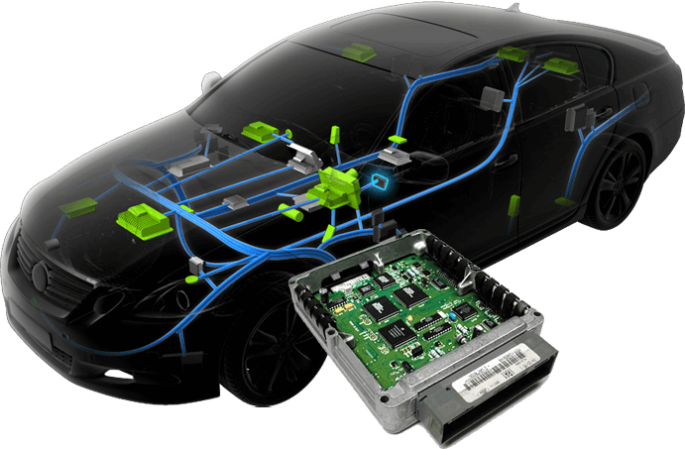
\includegraphics[width=0.5\textwidth]{imagenes/ECU_autotechdrive.png}
    \caption{Imagen de una ECU y su impacto en un vehículo. Extraído de: []}
\end{figure}


\subsection{Evolución e historia de la gestión de datos los vehículos}

Las siglas ECU no siempre han tenido el mismo significado. Inicialmente, cuando se comenzaron a utilizar (en torno a los años setenta), era para hablar de la unidad de control del motor \textit{\textbf{Engine Control Unit}}. Podemos desgajar los grandes cambios en lo siguiente[4]:

\begin{itemize}

    \item \textbf{Años 70} - Inicialmente eran dispositivos extremadamente simples, que solamente controlaban un par de solenoides en el \textbf{carburador}, el encargado de preparar la mezcla de aire y combustible en motores de gasolina, de manera que el vehículo pudiera obtener la máxima potencia de salida de la manera más eficiente.

    \begin{figure}[h]
        \centering
        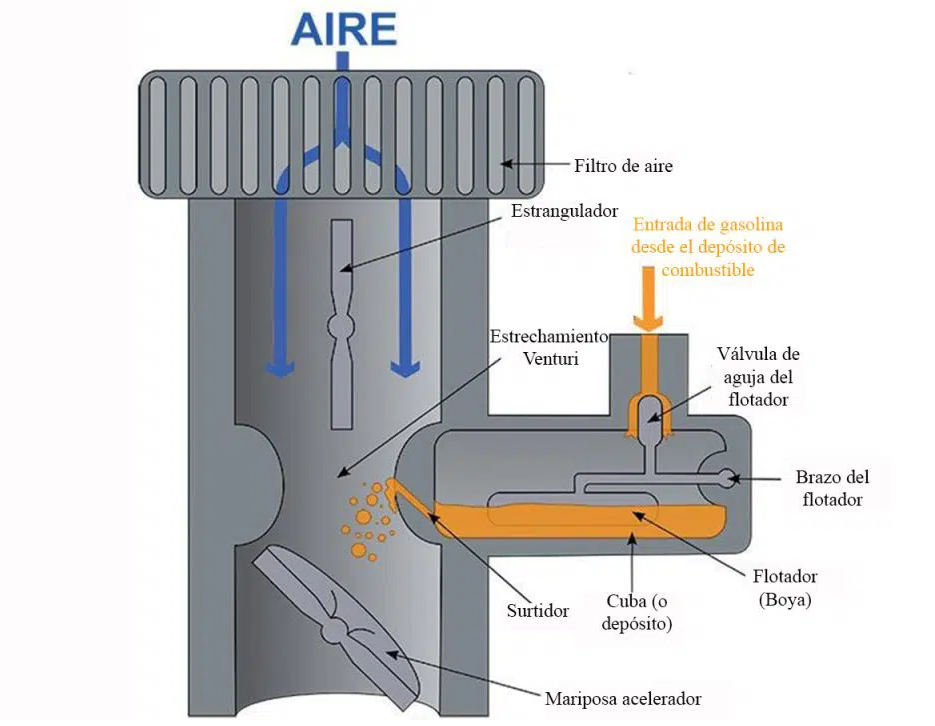
\includegraphics[width=0.5\textwidth]{imagenes/esquema_carburador.png}
        \caption{Imagen simplificada de un carburador sus partes. Extraído de: [5]}
    \end{figure}
 
    \item \textbf{Años 80} - En esta época se comenzaron a utilizar los \textbf{reguladores de presión de combustible}, un componente que busca controlar y mantener constante la presión del combustible. Permitió a los fabricantes de vehículos tener mayor control a la hora de no dañar otros componentes, tales como inyectores o los conductos del sistema en general [5]. En este punto, la unidad de control del motor ya era la principal responsable de los sistemas de combustión. También comenzaron a utilizar el \textbf{Control de Lambda} para modificar parámetros de la misma, y alcanzar una mayor eficiencia.

    \begin{figure}[h]
        \centering
        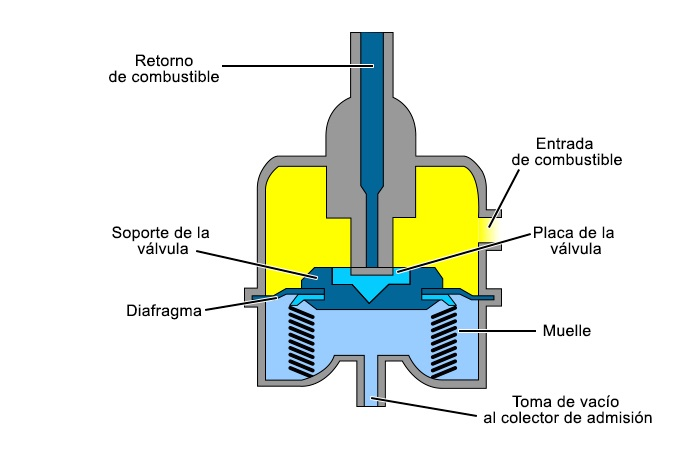
\includegraphics[width=0.6\textwidth]{imagenes/esquema_rpc.png}
        \caption{Imagen simplificada de un regulador de combustible y sus partes. Extraído de: [7]}
    \end{figure}


    \item \textbf{Años 90} - Las ECUs añadieron un conjunto de medidas para mejorar la seguridad en el vehículo, siendo el \textbf{ABS ó Antiblockiersystem} la más relevante. Esta tecnología, aún en uso en los vehículos actuales, se encarga de variar la fuerza de frenado al detectar mediante sensores de revoluciones en las ruedas, evitando así que estas se bloqueen y perdamos el control del vehículo. El uso de las ECUs se extiende hacia los motores diésel, teniendo un papel esencial en el desarrollo de los vehículos turbodiésel.

    \begin{figure}[h]
        \centering
        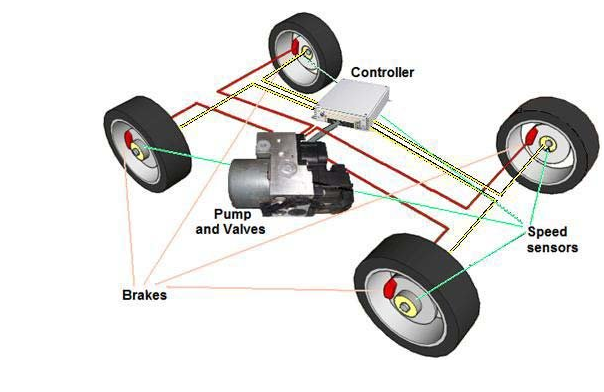
\includegraphics[width=0.5\textwidth]{imagenes/esquema_abs.png}
        \caption{Imagen simplificada del ABS y sus partes. Extraído de: [8]}
    \end{figure}
    
 
    \item \textbf{Años 2000} - Las unidades de control comienzan a incluir la tecnología \textit{\textbf{drive-by-wire}}, un formalismo para definir la sustitución de controles mecánicos tradicionales por sistemas electrónicos [9], así como también se añade control del turbo y sistemas para minimizar emisiones y cumplir con los protocolos pertinentes.
       

    \begin{figure}[h]
        \centering
        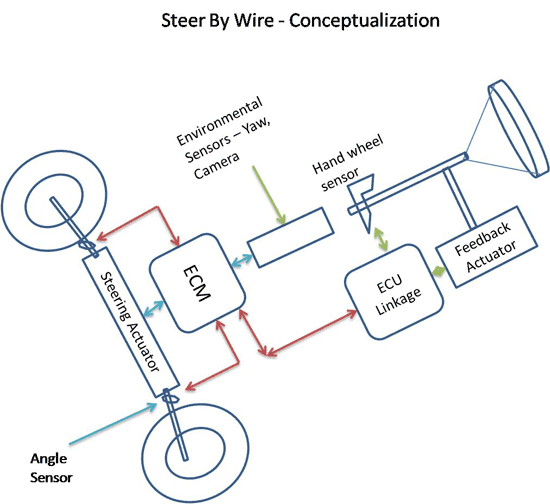
\includegraphics[width=0.5\textwidth]{imagenes/esquema_dbw.png}
        \caption{Conceptualización del sistema \textit{drive-by-wire}. Extraído de: [10]}
    \end{figure}
          

    \item \textbf{Años 2010-Actualidad} - La centralita del motor controla todo el sistema de mezcla del combustible, emisiones, refrigeración y sistemas de aceleración del vehículo. Dejan de ser dispositivos simples, ahora tienen cientos de entradas, decenas de sensores, y forman parte de un conjunto de ECUs (ya utilizando la acepción actual del término: \textit{Electronic Control Unit}), cada una focalizada en un conjunto de tareas, yendo desde el propio control del motor, hasta los sistemas de infoentretenimiento del vehículo. 
       

    \begin{figure}[h]
        \centering
        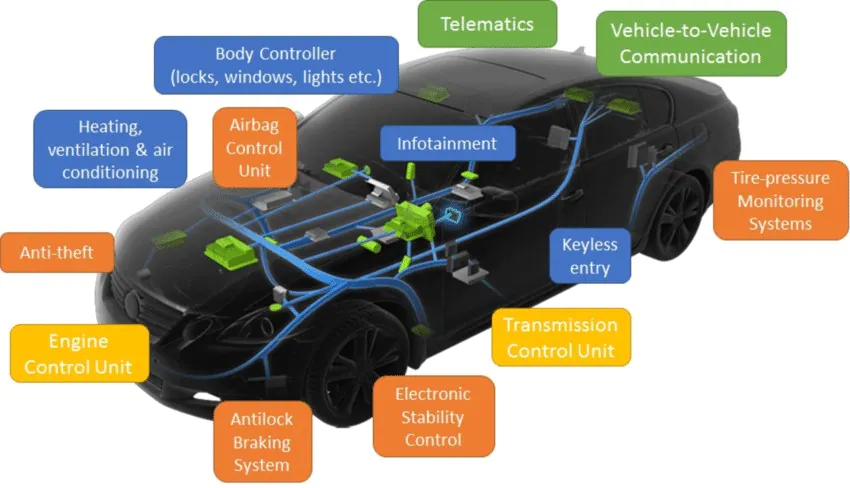
\includegraphics[width=0.5\textwidth]{imagenes/ECU_autotechdrive_completa.png}
        \caption{Representación de las distintas ECUs que controlan un vehículo. Extraído de: [11]}
    \end{figure}
\end{itemize}

\newpage
       
\begin{figure}[h]
    \centering
    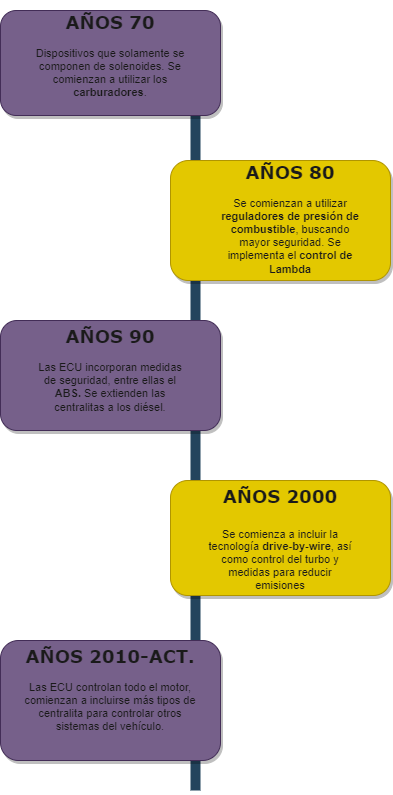
\includegraphics[width=0.54\textwidth]{imagenes/timeline_ECU.png}
    \caption{Linea temporal de las ECUs. Elaboración propia}
\end{figure}


\newpage


\subsection{Tipos de ECUs}
Como se ha visto en el anterior apartado, el significado de las siglas ECU ha variado con el tiempo, refiriéndose ahora a cada uno de los sistemas que controlan diversas partes del vehículo. A grandes rasgos, podemos hablar de los siguientes tipos[12]
\begin{itemize}
    \item \textbf{BCM - \textit{Body Control Module}}: Esta unidad controla tareas de índole variada, desde las luces, hasta el mecanismo de las ventanas, los retrovisores (si son motorizados), limpiaparabrisas, etc.
    \item \textbf{CCM - \textit{Climate Control Module}}: Este módulo se encarga de gestionar toda la climatización, temperatura, potencia de la bomba del aire acondicionado y calefacción.
    \item \textbf{ECM - \textit{Engine Control Module}}: Conocido antiguamente como ECU. Se encarga de gestionar todas las tareas del motor, ya mencionadas en el apartado anterior.
    \item \textbf{EBCM - \textit{Electronic Brake Control Module}}: Si el vehículo tiene un freno electrónico, este módulo es el encargado de su correcto funcionamiento.
    \item \textbf{ICM - \textit{Infotainment Control Module}}: Esta ECU controla todo lo relacionado con el infoentretenimiento, mayormente centrado en la tableta integrada del vehículo.
    \item \textbf{PSM - \textit{Power Steering Module}}: Este módulo gestiona las tareas que requiere la dirección para funcionar. Tiene una gran importancia, debido al uso de la dirección asistida en los vehículos actuales.
    \item \textbf{PCM - \textit{Powertrain Control Module}}: Esta ECU se encarga de la interconexión e interacción de los componentes que forman el \textbf{tren motriz}, el sistema que permite que la energía generada se transforme en movimiento sobre el terreno. Gestiona lo relacionado con el motor, la transmisión, los ejes, los diferenciales y la dirección del vehículo. 
    \item \textbf{SCM - \textit{Suspension Control Module}}: El objetivo de este módulo es controlar los sistemas de suspensión del vehículo.
    \item \textbf{TCM - \textit{Transmission Control Module}}: Este módulo controla todo lo relacionado con la transmisión, las marchas, el cambio y la entrega de potencia en las ruedas.
\end{itemize}
\newpage
\section{Diseño hardware de las centralitas}

Para tener un funcionamiento acorde a su importancia, las ECUs están constituidas por varios componentes, que serán los que se estudiarán en este apartado.

\begin{figure}[h]
    \centering
    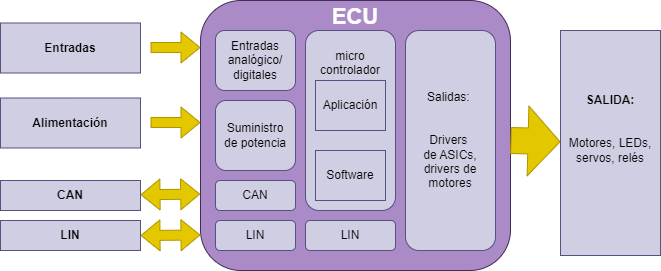
\includegraphics[width=0.70\textwidth]{imagenes/ECU_hardware.png}
    \caption{Componentes hardware de una ECU. Elaboración propia}
\end{figure}

\subsection{Procesador central}
El microcontrolador es la piedra angular de una centralita. Su tarea varía según el tipo de ECU que lo contenga, pero generalmente consiste en realizar todo el procesamiento de datos, así como hacer uso de las lineas de comunicación para recibir y enviar información a los subsistemas requeridos. \newline
Estos microcontroladores pueden interaccionar entre sí, aun perteneciendo a diferentes centralitas, por medio de \textbf{multiplexación}, así como también de los buses o protocolos de comunicación. Esta relación permite a un sistema valerse de otros para realizar una tarea, véase el siguiente ejemplo: 

\begin{enumerate}
    \item El usuario nota que hace demasiado calor en el vehículo, por lo que decide cambiar la temperatura en la tableta central del vehículo.
    \item Este sistema, controlado por el \textbf{ICM} (\textit{Infotainment Control Module}), recibe la entrada del usuario y envía una señal a la ECU que se encarga de la climatización (\textbf{CCM}).
    \item El módulo de climatización recibe la entrada y envía una señal a sus actuadores para encender el aire acondicionado.
\end{enumerate}


Respecto a la arquitectura del microcontrolador, existen diversas opciones, todas (o casi todas) ellas oscilando entre los 8 bits y los 32 bits, siendo estos últimos los más extendidos con el \textbf{Infineon Tri-core Microcontroller[19]}. Este micro se encarga de gestionar todas las tareas de emisiones y sistemas de combustión. 

La elección entre un chip u otro también se hace en base a las necesidades del sistema, puesto que algunos, como el tren de potencia y el control del vehículo requieren de un menor tiempo de respuesta y un mayor rendimiento, mientras que el infoentretenimiento no tiene tanta restricción al ser un \textbf{sistema de tiempo real blando} (incumplir el límite acotado del tiempo de respuesta no ocasiona daños personales o materiales)

\subsection{Memoria}

En una ECU, normalmente existen tres tipos de memoria, \textbf{ROM}, \textbf{RAM} y \textbf{PROM/EEPROM}. Cada una tiene un objetivo específico y unas restricciones asociadas:

\begin{itemize}
    \item \textbf{Memoria no volátil}: La ECU almacena en este tipo de memoria información que no se debe borrar una vez se apague el vehículo, como los datos del sistema y los del usuario (configuraciones, perfiles de conducción, etcétera.).
    \begin{itemize}
        \item \textbf{ROM}: Almacena información de programación que solo puede leer la ECU. Es de solo lectura, y su existencia es de vital importancia para el funcionamiento del vehículo.
        \item \textbf{PROM/EEPROM}: Este tipo de memoria está hecha por el fabricante, con el objetivo de ajustarse a la aplicación de la transmisión, motor y demás piezas fundamentales del vehículo. Mientras que la PROM no se puede reprogramar, la EEPROM (\textit{Electrically Erasable Programmable Read-Only Memory}) permite al usuario o al operario reprogramarla con un dispositivo especial. 
    \end{itemize}
    \item \textbf{Memoria volátil}: La ECU utiliza esta memoria para almacenar datos temporales, no mantiene la información entre reinicios.
    \begin{itemize}
        \item \textbf{RAM}: Esta memoria permite almacenar datos temporales de las entradas, códigos de error para el diagnóstico, y resultados de cómputos para trabajar con los actuadores. Tiene un tiempo de acceso mucho menor a las \textbf{NVM} (\textit{Non-Volatile Memory}).
    \end{itemize}
\end{itemize}

\subsection{Sensores}

Los sensores tienen un papel esencial en el diseño hardware de las ECU, dando información de los sistemas del vehículo al microcontrolador para su monitorización. 


\section{La ECU en los vehículos: El mejor amigo del conductor}

El ser humano ha hecho grandes avances en la tecnología, y esto no podría ser menos en los vehículos. Las ECU que, como se ha visto en el apartado anteror, inicialmente no tenían tanta importancia, ahora se han convertido en algo fundamental para nosotros. Estas centralitas, que antiguamente servían únicamente para gestionar la inyección de combustible en el el motor, ahora tienen multitud de utilidades para cada una de las partes del vehículo.

Gracias a estos sistemas, podemos obtener desde una mayor eficiencia en el uso de la fuente de energía (ya sea combustible fósil o electricidad), un control más específico de los mapas motor para mayor potencia, recolección de datos relevantes del vehículo, e incluso algunas mejoras \textit{Quality of Life (QoL)} que nos permitan una conducción más cómoda. 

Muchos de estos sistemas no solamente inciden en la eficiencia y comodidad, sino también en la seguridad del conductor y de los pasajeros abordo. Algunas de las medidas más relevantes, que vamos a categorizar entre activas y pasivas, son las siguientes[11]:

\begin{enumerate}
    \item \textbf{Seguridad activa} - Conjunto de medidas que proporcionan mayor estabilidad al vehículo, buscando evitar el accidente a priori.
    \begin{itemize}
        \item \textit{Luces adaptativas}: Esta tecnología se basa en el uso de una matriz de LEDs en las luces delanteras, al contrario de la tradicional bombilla incandescente usada anteriormente. Los beneficios de este diseño son múltiples, pues permite modificar el haz de luz para evitar posibles deslumbramientos a otros usuarios de la vía, así como también adaptarse a las condiciones de la carretera, e iluminar más eficazmente el trazado.


     
        \item \textit{Control de crucero adaptativo (ACC)}: Permite mantener una velocidad designada por el conductor, variando cuando sea necesario por las condiciones del tráfico. Esta tecnología supone una gran ayuda en el caso de que exista una distracción del conductor. Puede funcionar junto a un sistema de detección de señales para no sobrepasar la velocidad máxima permitida en esa vía.
    
        \item \textit{Sistema de alerta de tráfico y evasión de colisión (TCAS)}: Este sistema tiene como tarea principal la detección de eventos en el tráfico que puedan causar un accidente, reaccionando (normalmente accionando de manera automática el freno), o advirtiendo al conductor para que sea él el que realice la acción pertinente para evitarlo.

        \item \textit{Sistema de detección de cansancio}: Algunos fabricantes [14] comienzan a implementar esta tecnología que, mediante sensores en la posición del conductor, o analizando su conducción, permite detectar si existen síntomas de cansancio o distracción. Normalmente muestran un aviso que se repite de manera continuada hasta que se realiza una parada. 
\end{itemize}

\begin{figure}[h]
    \centering
    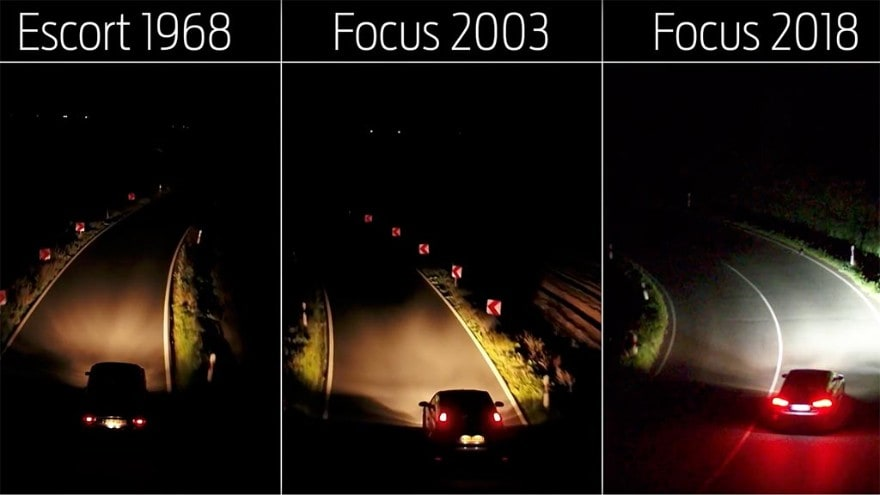
\includegraphics[width=0.7\textwidth]{imagenes/adaptive_lights.png}
    \caption{Comparación de la iluminación en los vehículos tras los años. Extraído de: [14]}
\end{figure}


    \item \textbf{Seguridad pasiva} - Conjunto de medidas que actúan una vez ha sucedido el accidente o el mal funcionamiento. Tienen el objetivo de minimizar los daños.

    \begin{itemize}
        \item \textit{Sistema de sensor de ocupación}: Permite detectar qué asientos están siendo utilizados, y comprobar el peso para saber si el ocupante es un niño o un adulto. Normalmente se utiliza para accionar el airbag si fuera necesario, y la altura a la que hacerlo.

        \item \textit{Notificación de colisión automática}: Este sistema envía un aviso a los servicios de emergencia de su localicación para que sea posible una intervención rápida.[16]
    \end{itemize}
\end{enumerate}




\section{La necesidad de un RTOS en las ECUs}

2.2.2 Real-Time Operating System
The general structure of a more recent (but not fully modern) ECU follows a model
similar to the main loops outlined in 2.2.1, but these loops are often distributed across
multiple cores with a more complex scheduling system. This requires the use of a realtime-operating-system (RTOS) to schedule, manage, and distribute the cores of the CPU so
that each function can execute on-time. This allows for important sensor reading functions,
health checking functions, and fuel injection functions to be ran concurrently, increasing
their speed and response time and greatly increasing their safety and optimizing their performance. Several contemporary open-source ECUs are implemented on top of an RTOS
to schedule necessary tasks, with a notable one being rusEfi which was built on top of the
open-source platform FreeRTOS[5]

\section{Futuras tendencias en el campo de las ECU: ¿Qué podemos esperar?}

\section{Código Abierto, Software Libre y Licencias}

El software libre y sus licencias \cite{gplv3} ha permitido llevar a cabo una expansión del
aprendizaje de la informática sin precedentes.

\section{Conclusiones}
	
	\chapter{Planificación}

\section{Metodología utilizada}


\section{Temporización}

\section{Seguimiento del desarrollo}


	% Análisis del problema
	% 1. Análisis de requisitos
	% 2. Análisis de las soluciones
	% 3. Solucion propuesta
	% 4. Análisis de seguridad
	\chapter{Análisis del problema}

\fancyhead[R]{6. Análisis del problema}

\noindent\fbox{
	\parbox{\textwidth}{
    En este capítulo se realizará un análisis algo más exhaustivo de la toma de diversas decisiones que afectarán al desarrollo del trabajo, véase los componentes, el sistema operativo de tiempo real, y demás componentes que conforman el proyecto y desarrollo. 
	}
}

\section{Elección de un sistema operativo}

\subsection{¿SO de propósito general o sistema operativo de tiempo real?}

El principal rol del sistema operativo es controlar los recursos del sistema para suplir las demandas de las aplicaciones que trabajan sobre él. Todos los SOs, independientemente de si son de propósito general o de tiempo real, tienen elementos esenciales tales como la planificación de procesos, control de memoria, relojes, entrada/salida, etcétera. 

Si bien comparten dichos elementos esenciales, los RTOS están diseñados con la filosofía de que sus tiempos de espera, procesamiento y respuesta son más importantes que su rendimiento promedio. Los RTOS se utilizan en los casos en los procesos deban estar planificados en el tiempo, garantizando que se cumplan los requerimientos temporales para dichos procesos. 

En el caso de este proyecto, se necesita que el SO a escoger tenga baja latencia, que pueda asegurar que las tareas que lo requieran terminarán en el tiempo determinado, así como permitir que las tareas críticas y no críticas coexistan en el sistema. También es muy importante que dicho SO tenga un sistema de asignación de prioridades que permita al programador establecer cuáles son las tareas y procesos más importantes para su proyecto y darles esa importancia en la ejecución.

\subsection{¿RTOS comercial o de código abierto?}

Si bien los RTOS comerciales ofrecen una mayor variedad de funciones para el programador, sus precios suelen ser demasiado elevados para poder escogerlos en un proyecto como este. Por ejemplo, en el caso de VxWorks, el RTOS propietario líder en el sector, de la empresa Wind River, el precio del SO comienza en los 18500\$ per seat (por usuario que trabaja con el sistema). Obviamente esto es algo prohibitivo para nuestro presupuesto, pero en el caso de una ECU que se implemente en vehículos sería la mejor opción.\newline

Pero no todos los RTOS son comerciales, sino que existen multitud de ellos que son de código abierto. A continuación se expone una tabla con las principales características de algunos de los RTOS \textit{open source} más importantes:

\begin{table}[H]
    \resizebox{\columnwidth}{!}{%
    \begin{tabular}{|l|l|l|l|}
    \hline
    \rowcolor[HTML]{CBCEFB} 
    \textbf{Nombre} &
      \textbf{Aplicación principal} &
      \textbf{\begin{tabular}[c]{@{}l@{}}Facilidad de \\ programación\end{tabular}} &
      \textbf{\begin{tabular}[c]{@{}l@{}}Eficiencia en \\ ECU\end{tabular}} \\ \hline
    \textbf{RIOT}        & \begin{tabular}[c]{@{}l@{}}Orientado a dispositivos de\\  Internet de las Cosas (IoT)\end{tabular} & Media   & Media \\ \hline
    \textbf{Nano-RK}     & \begin{tabular}[c]{@{}l@{}}Sistemas embebidos en\\ tiempo real\end{tabular}                        & Difícil & Alta  \\ \hline
    \textbf{FreeRTOS}    & \begin{tabular}[c]{@{}l@{}}Sistema operativo de tiempo\\  real de código abierto\end{tabular}      & Media   & Media \\ \hline
    \textbf{ARM mbed OS} & Plataforma de desarrollo para IoT                                                                  & Fácil   & Alta  \\ \hline
    \textbf{Raspbian}    & \begin{tabular}[c]{@{}l@{}}Sistema operativo general\\  para Raspberry Pi\end{tabular}             & Fácil   & Baja  \\ \hline
    \textbf{DuinOS}      & \begin{tabular}[c]{@{}l@{}}RTOS diseñado específicamente\\  para Arduino\end{tabular}              & Fácil   & Baja  \\ \hline
    \textbf{mipOS}       & \begin{tabular}[c]{@{}l@{}}RTOS de código abierto para\\  sistemas embebidos\end{tabular}          & Media   & Baja  \\ \hline
    \end{tabular}%
    }
    \caption[Selección de RTOS]{Lista de sistemas de tiempo real y sus características. Elaboración propia}

    \end{table}

Para escoger, comenzamos por descartar todos aquellos sistemas operativos que se utilicen para IoT, pues normalmente las restricciones de tiempo en esos sistemas son mucho más suaves. Si hacemos un balance entre la facilidad de programación y la eficiencia, pues el tiempo de desarrollo es bastante limitado y diseñar un programa en los sistemas más difíciles puede requerir demasiado tiempo, encontramos que la mejor alternativa es FreeRTOS. 

\subsubsection{FreeRTOS}

FreeRTOS es uno de los RTOS más utilizados para microcontroladores y pequeños microprocesadores, con soporte para una gran variedad de placas\cite{freertos}. Tiene una proyección \textbf{LTS} (\textit{Long Term Support}), lo que garantiza que el proyecto podrá seguir teniendo soporte a largo plazo. Una de sus grandes ventajas es la gran cantidad de librerías modulares, así como también el enfoque del kernel para ahorrar energía y no ser demasiado pesado. 

Por todas estas razones, FreeRTOS es la elección perfecta para un proyecto con estas características. 

\section{Elección de la placa}
\subsection{Requisitos}
A la hora de escoger la placa existen varios requisitos básicos debe cumplir, nombrados a continuación: 

\subsubsection{Soporte de FreeRTOS}

El primer requisito es que FreeRTOS soporte la placa que vayamos a escoger. Por suerte, este SO está ampliamente compatibilizado y existen multitud de placas disponibles\cite{freertos_comp}. Entre ellos están las placas de Altera, Infineon, Raspberry Pi, e incluso los usuarios han desarrollado FreeRTOS compatible con Arduino.

\subsubsection{Precio}

Si bien algunas de las placas anteriormente nombradas son objetivamente mejores, el presupuesto es limitado y requerimos de una placa que, como precio máximo, cueste 50\$. Con esto descartamos las placas de Altera e Infineon, así como una gran multitud de marcas que están orientadas a proyectos de ámbito profesional. 

\subsubsection{Rendimiento y frecuencia de reloj}

Al ser un proyecto con RTOS, se necesita que la placa tenga una frecuencia de reloj que permita realizar las funciones más importantes en un periodo corto, incluso en el peor caso. Para comenzar con la estimación, debemos destacar aquellas funciones del sistema que tengan el plazo más restrictivo. 

En el caso de la comprobación de la temperatura de batería y motor, debe de medirse dicha temperatura cada muy poco tiempo, asegurando así que el sistema no se esté sobrecalentando y pueda provocar un problema. 

Para realizar dichas mediciones, tendremos en cuenta dos funciones necesarias. 

\begin{enumerate}
    \item Inicio del sensor: Los sensores que se utilizan para medir temperaturas tienen un tiempo mínimo de 1s para conseguir la temperatura correcta, por lo que se iniciará y, un segundo después, se avisará a la segunda función.
    \item Comprobación de la temperatura: La ECU leerá los valores que le ha mandado el sensor en el último segundo y, mediante una ecuación, hallará el valor en grados celsius correspondiente. Tras hacer esto, comparará el valor con el límite superior que definen el intervalo de temperaturas correctas y, si no está dentro de dichos valores, enviará una señal a otra función que mostrará el aviso de temperatura por pantalla. 
\end{enumerate}

La segunda función es la que nos marcará el mínimo valor necesario de frecuencia de reloj para que el sistema pueda funcionar correctamente, realizando mediciones cada 100 ms. Para poder hallar entonces cuál es ese valor, programamos con pseudocódigo de manera básica una función que realice el proceso:


Se ha tomado como referencia un sensor LM35 cuya ecuación para hallar la temperatura es la siguiente: 

\begin{verbatim}
    Temperatura = Valor * 5 * 100 /1024
\end{verbatim}


\begin{verbatim}
    subproceso funcion temperatura_bateria
        tempB <- leer(sensor)
        temB <- (tempB * 5 * 100) / 1024
        si tempB > 45
            entonces temp_error = 1
        fin si
    fin funcion
\end{verbatim}

Teniendo ya este pseudocódigo, podemos estimar de manera aproximada la cantidad de ciclos y las instrucciones necesarias para llevar a cabo esta función, por lo que necesitamos convertir este código a ensamblador: 

\begin{verbatim}
    LDR rdi, #SENSOR 
    MUL $0.48828125, rdi
    CMP rdi, $45
    JA .L1
    MOV $1, rsi

    .L1
\end{verbatim}

Por motivos de eficiencia se ha reducido la operación de la fórmula al mínimo posible. 

Teniendo en cuenta que la operación que mayor número de cicos necesita, que es LOAD, con cinco ciclos, vamos a aproximar el número de ciclos del resto de instrucciones a 5 para poseer mayor margen en el cálculo a la hora de escoger la frecuencia de reloj necesaria.

Por tanto, nuestro programa tardará como mínimo 5 * 5 = 25 ciclos de reloj.

Ahora, teniendo en cuenta lo aprendido en la asignatura de Arquitectura de Computadores, vamos a hallar la frecuencia de reloj mínima para que el sistema pueda realizar este proceso en el tiempo determinado de 10ms. Utilizaremos la siguiente fórmula: 

\begin{align*}
    T_{CPU} = NI * CPI * T_{CICLO}
\end{align*}

Añadiendo los datos que conocemos, resolvemos la ecuación:

\begin{align*}
    100ms = 5 * 5 * T_{CICLO} 
\end{align*}

\begin{align*}
    \frac{100}{25} = T_{CICLO}
\end{align*}


\begin{align*}
    T_{CICLO} = 4ms
\end{align*}

Si calculamos la inversa del tiempo de ciclo, obtenemos la frecuencia mínima a la que debe operar nuestra placa para poder cumplir con los requerimientos:\newline
\begin{align*}
    Frecuencia > \frac{1}{0.04s}
\end{align*}

\begin{align*}
    Frecuencia > 2.5kHz
\end{align*}

\subsubsection{Periféricos}

Por último, se valorará que la placa tenga los siguientes parámetros:

\begin{itemize}
    \item Número de entradas/salidas digitales
    \item Salidas analógicas con \textbf{PWM} (pulse width modulation)
    \item Comunicación \textbf{I2C}(Inter-Integrated Circuit)
    \item Puertos serie
\end{itemize}



\subsubsection{Conclusiones}

Una vez analizados los puntos más importantes, se ha seleccionado una variedad de placas que cumplen uno o varios requisitos nombrados. 

\begin{table}[H]
    \resizebox{\columnwidth}{!}{%
    \begin{tabular}{|l|l|l|l|l|l|l|l|}
    \hline
    \rowcolor[HTML]{ECF4FF} 
    \textbf{Nombre} &
      \textbf{Empresa} &
      \textbf{\begin{tabular}[c]{@{}l@{}}Frecuencia \\ Reloj\end{tabular}} &
      \textbf{RAM} &
      \textbf{\begin{tabular}[c]{@{}l@{}}Utilidades \\ Incluidas\end{tabular}} &
      \textbf{\begin{tabular}[c]{@{}l@{}}Soporta \\ FreeRTOS\end{tabular}} &
      \textbf{\begin{tabular}[c]{@{}l@{}}Temperatura \\ de Operación\end{tabular}} &
      \textbf{PVP} \\ \hline
    \textbf{Arduino Mega 2560} &
      Arduino &
      16 MHz &
      8 KB &
      \begin{tabular}[c]{@{}l@{}}UART, SPI, I2C, \\ PWM, ADC\end{tabular} &
      Sí* &
      -40°C a 85°C &
      40\$ \\ \hline
    \textbf{Raspberry Pi 4} &
      \begin{tabular}[c]{@{}l@{}}Raspberry Pi\\  Foundation\end{tabular} &
      1.5 GHz &
      4 GB &
      \begin{tabular}[c]{@{}l@{}}GPIO, UART, \\ SPI, I2C, PWM, \\ ADC\end{tabular} &
      Sí &
      0°C a 50°C &
      45\$ \\ \hline
    \textbf{\begin{tabular}[c]{@{}l@{}}BeagleBone \\ Black\end{tabular}} &
      BeagleBoard.org &
      1 GHz &
      512 MB &
      \begin{tabular}[c]{@{}l@{}}GPIO, UART, \\ SPI, I2C, ADC\end{tabular} &
      Sí &
      -20°C a 85°C &
      55\$ \\ \hline
    \textbf{Teensy 4.1} &
      PJRC &
      600 MHz &
      1024 KB &
      \begin{tabular}[c]{@{}l@{}}UART, SPI, I2C, \\ PWM, ADC\end{tabular} &
      Sí &
      -40°C a 85°C &
      32\$ \\ \hline
    \textbf{\begin{tabular}[c]{@{}l@{}}STM32 \\ Nucleo-F767ZI\end{tabular}} &
      STMicroelectronics &
      216 MHz &
      512 KB &
      \begin{tabular}[c]{@{}l@{}}UART, SPI, I2C, \\ PWM, ADC\end{tabular} &
      Sí &
      -40°C a 85°C &
      52\$ \\ \hline
    \textbf{\begin{tabular}[c]{@{}l@{}}NVIDIA \\ Jetson Nano\end{tabular}} &
      NVIDIA &
      1.43 GHz &
      4 GB &
      \begin{tabular}[c]{@{}l@{}}GPIO, UART, \\ SPI, I2C, USB, \\ Ethernet, HDMI\end{tabular} &
      Sí &
      0°C a 50°C &
      99\$ \\ \hline
    \textbf{\begin{tabular}[c]{@{}l@{}}PSoC 6 \\ BLE Pioneer Kit\end{tabular}} &
      \begin{tabular}[c]{@{}l@{}}Cypress \\ Semiconductor\end{tabular} &
      150 MHz &
      1 MB &
      \begin{tabular}[c]{@{}l@{}}UART, SPI, I2C, \\ PWM, ADC\end{tabular} &
      No &
      -40°C a 85°C &
      49\$ \\ \hline
    \end{tabular}%
    }
    \caption[Selección de placa]{Lista de placas seleccionadas y sus características. Elaboración propia}

    \end{table}

    Teniendo en cuenta esta tabla, comenzamos a descartar aquellos que superen el presupuesto inicial de 50\$. Después, aquellas que no tengan soporte para FreeRTOS. La elección final, entre la placa Teensy y la arduino mega, es mayormente por la documentación y el soporte que tengan las placas. Se ha escogido la \textbf{Arduino Mega 2560} porque, además de dicha documentación, facilita el montaje del prototipo gracias a sus pines, evitando así la necesidad de soldar ni de una protoboard. Otra razón de peso para elegir esta tecnología es que tiene un conocimiento avanzado de Arduino debido a las asignaturas cursadas en la carrera, así como por proyectos realizados de manera autónoma durante el transcurso de la misma, por lo que reducirá los tiempos de aprendizaje y programación. 

 \section{Elección de software para la interfaz}

 A la hora de escoger una alternativa para crear interfaces de usuario, existen multitud de opciones válidas. Se ha estudiado la viabilidad de utilizar HTML, CSS y JavaScript para el desarrollo, pero se ha descartado por la complejidad a la hora de implementar la comunicación con el puerto serie, así como por la curva de dificultad y desconocimiento de JavaScript. También se ha planteado utilizar un Framework como React o Angular, pero han sido descartados por la razón anterior, y el tiempo que conllevaría aprender estas tecnologías. 

 Por otra parte, Processing, una herramienta que se basa en el lenguaje Java, tiene mayor facilidad de implementación en proyectos de escala media-baja, como es el que se está realizando, así como también multitud de librerías que incluyen recursos útiles sin necesidad de realizarlos desde cero. Si bien no es el software más potente, cumple con su función y es la opción sencilla de utilizar, teniendo en cuenta que el foco central de este trabajo no es la creación de la GUI. 

 A la hora de escoger la librería se han revisado varias opciones, como PUI y G4P, pero ambas carecían de visualización de temperaturas y estaban más orientadas a la creación de gráficos 3D, por lo que se ha optado por ControlP5. 

 ControlP5\cite{controlP5} es una librería desarrollada por Andreas Schlegel, que basa su uso en la creación de gráficos sencillos para interfaces de usuario, tales como botones, visualizadores de valores y ruedas o \textit{knobs} para variar valores. Es una herramienta de fácil implementación y aprendizaje, con multitud de alternativas de uso, y que posee todo lo necesario para realizar la GUI de este proyecto. 
 
\section{Elección de periféricos}
 
Si bien no es una parte tan importante de la selección de componentes, escoger un buen periférico puede facilitar las labores de montaje y programación. No todos los periféricos pueden ser válidos en este proyecto, pues existen restricciones de precio y tamaño, por lo que se tiene que tener en cuenta estos parámetros a la hora de escoger. 



 \subsection{Motor}

 En el caso de los motores, existen tres tipos principales: 

 \begin{enumerate}
  \item Motores DC: Son los más utilizados, aunque pueden requerir de un módulo de control o un puerto PWM para poder ser manejados con eficiencia.
  \item Motores paso a paso: Giran mediante pasos, siendo 1.8º y 3.75º las medidas más usuales. Requieren de un módulo para controlar su manejo.
  \item Servomotores: Son motores que únicamente pueden dar un giro de 180º, pero proporcionan un control total del giro.
 \end{enumerate}

 En este caso, la elección ha sido clara, los motores DC cumplen con todo lo necesario y además existen multitud de modelos. 
 Se ha escogido un motor básico, con eje para conectarse a la rueda, y se comprarán dos unidades para las dos ruedas delanteras del vehículo. 

 \subsubsection{Placa de control de motor}

 Entre las dos alternativas más utilizadas, el driver L298H, con una capacidad para dos motores DC, y el escudo L293D, de la empresa MH Electronics, se ha escogido el primero debido a haber trabajado con el anteriormente y conocer su funcionamiento, además de ser apto para los dos motores DC necesarios. 

 \begin{figure}[H]
  \centering
  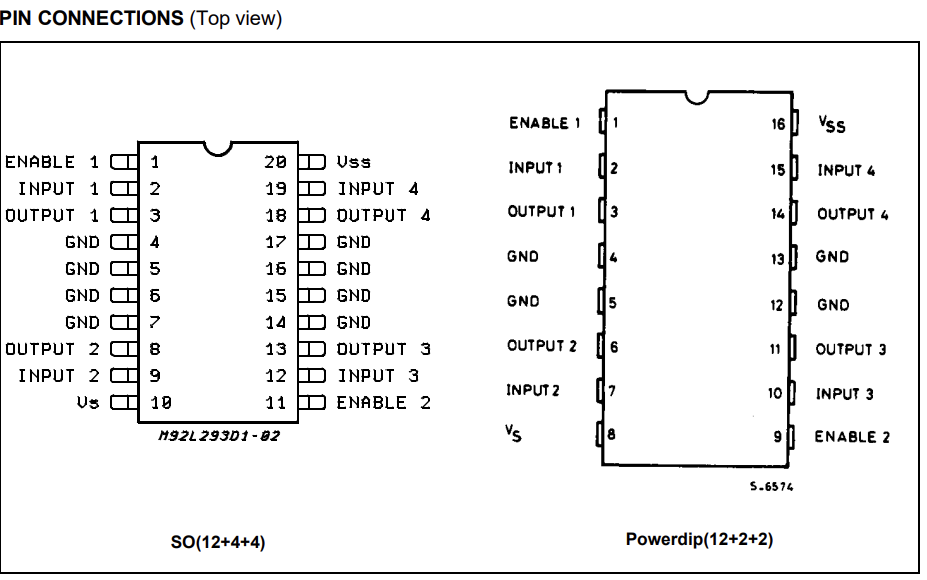
\includegraphics[width=1\textwidth]{imagenes/pinout_L293D.png}
  \caption{Esquema de pines del Shield L293D. Extraído de: [27]}
\end{figure}

 \subsection{Sensores de temperatura}

 Respecto a los sensores de temperatura, se ha escogido el termistor MF52 de 10K Ohm, debido a su bajo coste y su buena precisión.
 Se comprarán dos, uno para la temperatura del motor y otro para la batería.

 \subsection{Batería}

 Como elección de las baterías, se ha escogido un pack de dos baterías recargables ENEGON, de 9 voltios y 650 miliamperios/hora, suficiente para suministrar energía a los motores. Además, es recargable por usb para una mayor utilidad.
 
\section{Componentes en situaciones reales}

Si bien estos componentes cumplen las necesidades del proyecto, nunca serían útiles en un entorno real. Esta ECU es una abstracción de una ECU real, en la que tendríamos que tener en cuenta muchos más factores tales como la temperatura, mayor fiabilidad en los sistemas, así como el resto de requerimientos que tendría un vehículo real, incluyendo un motor de gasolina que complicaría el sistema y conlleva multitud de riesgos. Además, los componentes que se utilizarían en un entorno real rondan los miles de euros, por lo que no es posible realizar un proyecto realista. 

	% Desarrollo bajo sprints: 
	% 	1. Permitir registros y login de usuarios
	% 	2. Desarrollo del sistema de incidencias
	% 	3. Desarrollo del sistema de denuncias administrativas y accidentes
	% 	4. Desarrollo del sistema de croquis
	%   5. Instalación de la aplicación de manera automática
	\chapter{Implementación}

La implementación del software se ha dividido en hitos. Estos, han sido definidos en Github
y cada uno de ellos contiene un grupo de \textit{issues} que se corresponden con las distintas
mejoras que se han ido incorporando al software a lo largo de su desarrollo.\\



	% Presupuesto

	% Conclusiones
	\chapter{Conclusiones y trabajos futuros}



	% Trabajos futuros


	
	\newpage
	\bibliography{bibliografia}
	\bibliographystyle{plain}
	
\end{document}

